%begin_custom_header
\documentclass[11pt]{article}	% RECOMB: "at least 11 point font size on U.S. standard 8 1/2 by 11 inch paper with no less than one inch margin all around."				
\usepackage[utf8]{inputenc}   % umlauts etc.
\usepackage[english]{babel}
\usepackage [autostyle, english = american]{csquotes}
\MakeOuterQuote{"}
\usepackage{hyperref}
\usepackage{array}
% ----------------------------------
\usepackage[backend=biber,style=nature,sorting=none,url=false]{biblatex}
% url = false. There are also isbn, doi etc., similar options. 
\addbibresource{/Users/mohammedalshamrani/Downloads/School/Waldispul/Publishing/z-misc/zotero-library/my_library.bib}
% ----------------------------------
% Citation style 	biblatex stylename
% ----------------------------------
% 	ACS				chem-acs
% 	AIP				phys (*)
% 	Natur			nature
% 	Science			science
% 	IEEE			ieee
% 	Chicago			chicago-authordate
% 	MLA				mla
% 	APA				apa
% ----------------------------------
% sorting options:
% ----------------------------------
%	nty 		Sort by name, title, year.
%	nyt 		Sort by name, year, title.
%	nyvt 		Sort by name, year, volume, title.
%	anyt 		Sort by alphabetic label, name, year, title.
%	anyvt 		Sort by alphabetic label, name, year, volume, title.
%	ynt 		Sort by year, name, title.
%	ydnt 		Sort by year (descending), name, title.
%	none 		Do not sort at all. All entries are processed in citation order.
% ----------------------------------
\newcommand{\harpoon}{\overset{\rightharpoonup}}
\newtheorem{theorem}{Theorem}
\usepackage{verbatim} % multiline comment
\usepackage{graphicx}
\graphicspath{{/Users/mohammedalshamrani/Downloads/School/Waldispul/Publishing/Paper_04/fig/}}
\setlength\fboxsep{0pt} % figure border padding
\setlength\fboxrule{1pt} % figure outline
\usepackage[fleqn]{amsmath}  % also \documentclass[fleqn]{article}
\usepackage[margin=1in]{geometry}
\abovedisplayskip=0pt
\abovedisplayshortskip=0pt
\belowdisplayskip=0pt
\belowdisplayshortskip=0pt
\setlength{\mathindent}{0pt}
\usepackage{amsfonts} % for R (real numbers)
\usepackage{float}
\usepackage[font=scriptsize,labelfont=bf]{caption}

\usepackage[percent]{overpic}
\usepackage[export]{adjustbox}
% ----------------------------------
%Squeezing the Vertical White Space
%http://www.terminally-incoherent.com/blog/2007/09/19/latex-squeezing-the-vertical-white-space/
% 	THIS FIXES THE PROBLEM OF SUBSECTIONS STARTING IN A NEW PAGE
\setlength{\parskip}{0pt}
\setlength{\parsep}{10pt}
\setlength{\headsep}{0pt}
\setlength{\topskip}{0pt}
\setlength{\topmargin}{0pt}
\setlength{\topsep}{0pt}
\setlength{\partopsep}{10pt}
\usepackage[compact]{titlesec}
\titlespacing{\section}{0pt}{*2}{*2} % {left margin} {above-skip} {below-kip} , The * notation replaces the formal notation using plus/minus and etc. 
\titlespacing{\subsection}{0pt}{*1}{*1}
\titlespacing{\subsubsection}{0pt}{*1}{*1}
% ----------------------------------
\newenvironment{absolutelynopagebreak}
  {\par\nobreak\vfil\penalty0\vfilneg
   \vtop\bgroup}
  {\par\xdef\tpd{\the\prevdepth}\egroup
   \prevdepth=\tpd}
% ----------------------------------
\newcommand{\bfl}{\begin{flushleft}}
\newcommand{\efl}{\end{flushleft}}
\newcommand{\mys }{\hspace{0.1cm}}
\newcommand{\figfont}{\footnotesize}

\title {\large Single-Primer Polymerase Chain Reactions }
\usepackage{authblk}
\author[1]{Ali Atiia}
%\author[2]{Silvia Vidal}
%\author[4]{François Major}
\author[1]{Jérôme Waldispühl}
\renewcommand\Authfont{\fontsize{9}{14}\selectfont}
\affil[1]{School of Computer Science, McGill University, Montreal, Canada}
%\affil[2]{Research Centre on Complex Traits, McGill University, Montreal, Canada}
%\affil[3]{National Institute of Informatics, Tokyo, Japan }
%\affil[4]{Institute for Research in Immunology and Cancer, Montreal, Canada}
\setcounter{Maxaffil}{0}
\renewcommand\Affilfont{\fontsize{7}{14}\selectfont} % the second number determines spacing between lines
%=================================================================================
\date{}
\usepackage[table]{xcolor} % for \arrayrulecolor{yellow}, changes hline and vline colors
\usepackage{array}
\usepackage{lmodern}
\usepackage{multirow, booktabs} % http://tex.stackexchange.com/questions/328793/table-custom-cell-vertical-alignment					
\usepackage{lmodern}
\usepackage{multirow, booktabs} % http://tex.stackexchange.com/questions/328793/table-custom-cell-vertical-alignment					
\begin{document}
	\maketitle
	\begin{abstract}
			
		% \tiny, \scriptsize, \footnotesize, \small, \normalsize, \large, \Large, \LARGE, \huge, and \Huge.
		
		 Polymerase chain reaction (PCR) is an indispensable molecular biology technique
		 used to selectively amplify a segment of DNA using a thermostable polymerase that extends two short oligonucleotides
		 that complement the 3' ends of the target sequence. The annealing of the two primers
		 to the target extremities at the same temperature is the most important factor in determining the success of the reaction,
		 as misannealing of either or both to non-target regions (or to themselves, "primer-dimer") can lead to erroneous 
		 ampilicons. Having different annealing temperatures can also hinder the success of the reaction, requiring the setting of the reaction
		 annealing temperature to the lowest of the two which can also lead to various problems. Primer design has therefore emerged
		 as one of the most important steps to ensure successful reactions with high yields. There exist many bioinformatic tools
		 to help achieve that, but in practice some primer pairs may still not work well together. Furthermore, when the GC content of 
		 the two extremeties are greatly different, it may become a difficult task to find a suitable primer pair, especially when
		 the choice of primer locations is limited. For example, one primer at one extremity may be a T7 promoter while the other 
		 is part of the coding sequence at another. Here we present a simple technique of inserting the complement of one primer into 
		 one extremity, thereby allowing the use of one primer to anneal to both extremeties of the target ampilicon, thereby 
		 eliminating the need to optimize the design or reaction conditions that suit two different primers. The involved procedure
		 employ standard molecular biology procedure (phosphorylation, digestion, and ligation) and does not require
		 any special sequence modification beside the insertion of one sequence. The method can simplify the engineering 
		 and mass production of plasmids and custom in-vitro transcription templates (for sure in gene (protein) design for example).
		 Designing the 2-way primer to have an annealing temperature equals to that of the extension also eliminates the need
		 for an annealing step during the cycling program of a reaction, resulting in a significant reduction of total reaction time.  
		 	
		\begin{comment}	
			applications:
				de novo gene (protein) design 
				plasmid preparations
			
			the diagnosis and monitoring of genetic diseases, identification of criminals (in the field of forensics), and studying the 
			function of a targeted segment of DNA.
		
			a variety of applications.[4][5] These include DNA cloning for sequencing, DNA-based phylogeny, or functional analysis of 
			genes; the diagnosis of hereditary diseases; the identification of genetic fingerprints (used in forensic sciences and DNA
			paternity testing); and the detection of pathogens in nucleic acid tests for the diagnosis of infectious diseases.
 		\end{comment}
	\end{abstract}
\newpage
%\section{Introduction} \label{intro}			
		%\parbox[t]{\textwidth}{At the intersection”}
		
		\begin{comment}
				\begin{figure}[h]
					%\begin{overpic}[width=0.5\textwidth,grid,tics=10]{algorithmic_workflow/algorithmic_workflow.pdf}
					%\begin{overpic}[width=16.5cm, height=15.5cm, right]{algorithmic_workflow/algorithmic_workflow_cropped.pdf}
					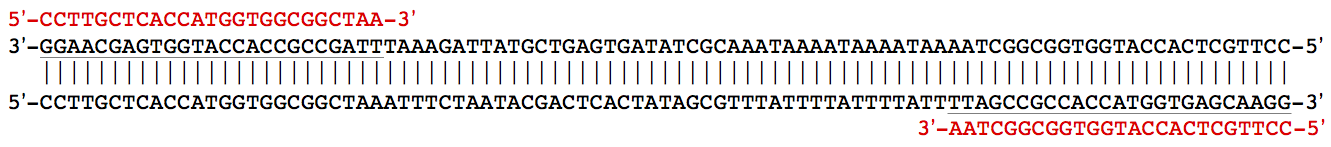
\includegraphics[scale=.5,center]{01_schematics/aseq.png} 
					%\includegraphics[scale=.3]{02.degree-dist/ER_Vinayagam.png}
					\caption{schematic}
					\label{fig:schematic}
				\end{figure}
		\end{comment}
		\begin{figure}[H]
			\begin{table}[H]
				\arrayrulecolor[HTML]{ffffff}% midrule is used to create vertical space between rows, make it white. blue = 0a84f7
				\centering
				% multirow is used to control vertical alignment within a cell: http://tex.stackexchange.com/questions/328793/table-custom-cell-vertical-alignment
				\begin{tabular}{{  | @{}p{.1cm} | p{12.5cm}@{} |   }}				
					\toprule
					\multirow{-4}{\linewidth}{\footnotesize{(1)}} & 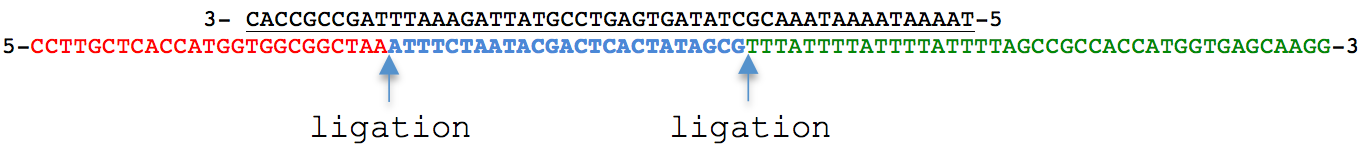
\includegraphics[scale=.25, center]{03_method/m1.png} 
					\\ \midrule\midrule\midrule\midrule  % midrule is thicker than \hline
					\multirow{-4}{\linewidth}{\footnotesize{(2)}} & 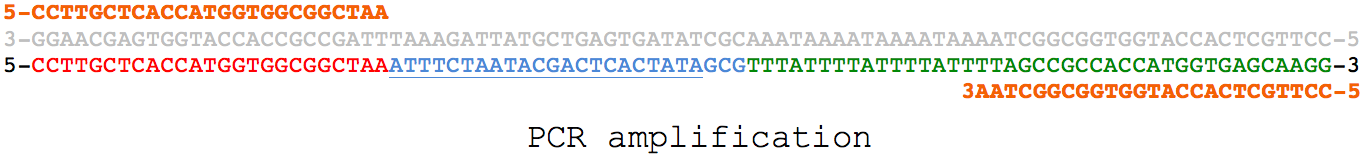
\includegraphics[scale=.25, center]{03_method/m2.png} 
					\\ \midrule\midrule\midrule\midrule  
					\multirow{-4}{\linewidth}{\footnotesize{(3)}} & 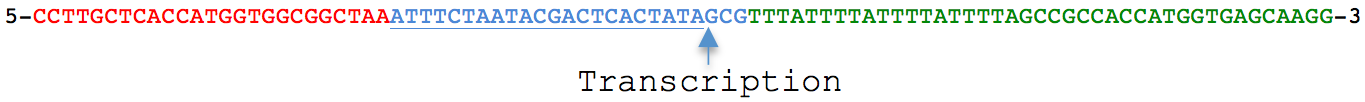
\includegraphics[scale=.25, center]{03_method/m3.png}  
					\\ \midrule\midrule\midrule\midrule  
					\multirow{-1}{\linewidth}{\footnotesize{(4)}} & 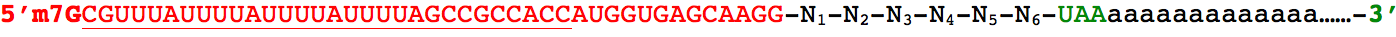
\includegraphics[scale=.25, center]{03_method/m4.png} 
					\\ \bottomrule
				\end{tabular}
			\end{table}		
			\caption{Construction of dsDNA templates}
			\label{fig:method}	
		\end{figure}

		
\section{Results} \label{sec:results}
			Here we present ultraviolet images of gel electrophoresis showing DNA templates, RNA transcript, and RNA ligation results. 
			Figure \ref{fig:results}  (a) and (b) show double-stranded DNA (dsDNA) templates encoding nodes N0 to N6 and 
			edges E0 $\rightarrow$E1 to E5 $\rightarrow$E6, respectively.  The inset shows the reference molecular marker (ladder) 
			used to verify that the observed length of each dsDNA template appears on the gel at the expected length. The PCR product of 
			N6 dsDNA template (Figure 4a, well 7 from the left) shows erroneous bands, so the correct band is gel-excised under ultraviolet 
			visualization and purified using the crush-and-soak method [28]. The transcription of N6 results in a clean band corresponding 
			to the expected length of 98-nt (well 8 in Figure 4b). RNA transcripts of E0$\rightarrow$E1, E1$\rightarrow$E2, E2$\rightarrow$E3, 
			E3$\rightarrow$E4, E4$\rightarrow$E5, and E5$\rightarrow$E6 in Figure 4b (wells 10-15) show smears as they are loaded immediately 
			from in-vitro transcription reaction without purification, while purified transcripts of N0 to N6  are purified prior to loading 
			(Zymo Research kit \# R1019). The length of an RNA transcript is the length of its corresponding DNA template minus the T7 
			promoter region (25-bp) and leading sequence (25-32 bp). For example, the length of N6’s RNA transcript 
			is 98-nt = 152 - 29 – 25 (152-bp total dsDNA template length – 29-bp (leading) –  25-bp T7 (promoter)).
			\begin{figure}[H]
				\begin{table}[H]
				    \arrayrulecolor[HTML]{ffffff}% midrule is used to create vertical space between rows, make it white. blue = 0a84f7
					\centering
					% multirow is used to control vertical alignment within a cell: http://tex.stackexchange.com/questions/328793/table-custom-cell-vertical-alignment
					\begin{tabular}{{  | @{}p{.6\textwidth} | p{.1\textwidth}@{} |   }}				
						\toprule
						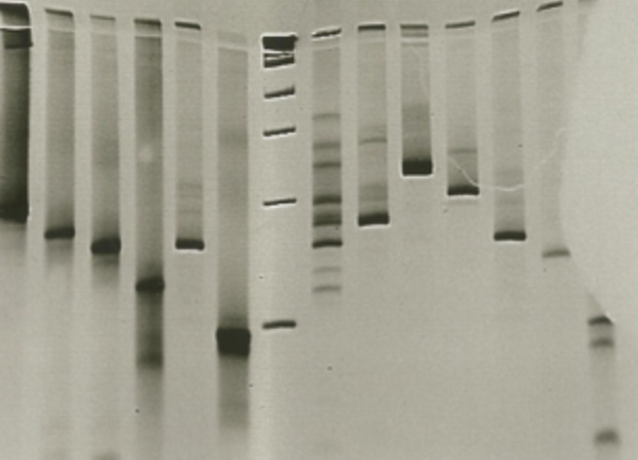
\includegraphics[scale=.75, center]{02_results/dsDNA.pdf}  
						& 
						\multirow{-10}{\linewidth}{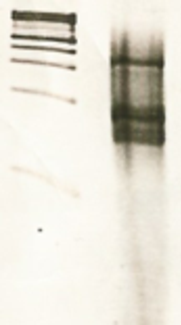
\includegraphics[scale=.6, center]{02_results/RNA_ligation.pdf} } 
						\\
						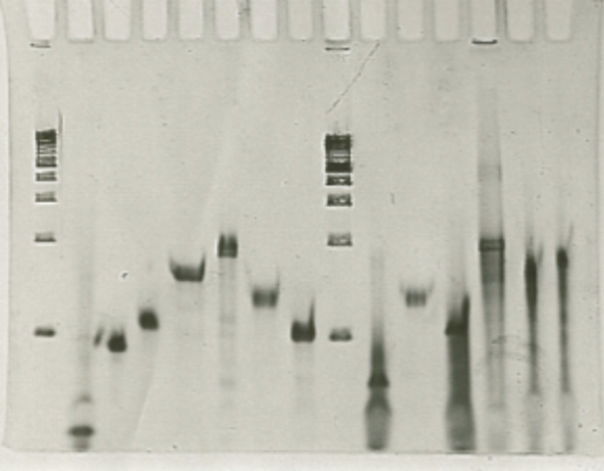
\includegraphics[scale=.75, center]{02_results/RNA.pdf}   
						& 
						\multirow{-10}{\linewidth}{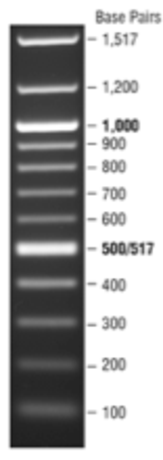
\includegraphics[scale=.5, center]{02_results/ladder.pdf}  }  
						%\\ \midrule\midrule\midrule\midrule  % midrule is thicker than \hline
						\\ \bottomrule
					\end{tabular}	
				\end{table}		
				\caption{Gel electrophoresis results of DNA templates, RNA transcripts, and RNA ligation products. 
							Inset: standard 100-bp molecular marker (NEB). (a) Double-stranded DNA (dsDNA) template strands encoding 
							for nodes \& edges, run on 4\% non-denaturing polyacrylamide gel. Wells left to right, w1-w7: templates 
							N0 to N6 of lengths 91, 134, 151, 194, 224, 170, and 152 base pairs (bp), respectively; w8: marker (inset); 
							w9-14: partial set of dsDNA templates encoding for edges E0$\rightarrow$E1, E1$\rightarrow$E2, E2$\rightarrow$E3, 
							E3$\rightarrow$E4, E4$\rightarrow$E5, and E5$\rightarrow$E6 of lengths 70, 123, 98, 182, 133, 149 bp, respectively.  
							N6 template (well 7) shows erroneous PCR byproducts subsequently excluded by excising the correct 
							band \& crush-and-soak purifying it [28]. Each sequence is primed upstream with a T7 promoter. 
							(b) Partial set of purified in-vitro transcribed RNA nodes \& edges run on 4\% TBE-Urea denaturing 
							polyacrylamide gel; left to right, w1/w9: marker (inset), w2-w8: RNA transcripts of N0 to N6 with 
							lengths 44, 87, 102, 147, 177, 120, 98-nt, respectively; w10-w15: RNA transcripts of edges E0$\rightarrow$E1, 
							E1$\rightarrow$E2, E2$\rightarrow$E3, E3$\rightarrow$E4, E4$\rightarrow$E5, and E5$\rightarrow$E6 
							with lengths 70, 123, 98, 182, 133, 149-nt, respectively. (c) Example RNA ligation; w1: marker (inset); 
							w2: ligation of N3 RNA transcript (147-nt) to N4 (177-nt) by splint ligation with edge 3$\rightarrow$E4 
							transcript (182-nt) to form a 324-nt RNA strand (ligation product). 
							}
				\label{fig:results}
			\end{figure}
\section{Method} \label{sec:method}
		%\parbox[H]{\textwidth}{
			DNA templates were constructed using ligation from smaller synthesized oligonucleotides (Biocorp). Segments of each 
			node/edge sequence were concatenated using splint ligation with T4 DNA ligase. The following example illustrates the 
			assembly and ligation of N0’s DNA template: 
			%\newline
			
			% insert figure
		
			The splint oligonucleotide (black, underlined) and the constituent oligonucleotides of a node (red, blue, and green) 
			were mixed at 10 uM concentration each in a 30-ul ligation reaction (50 mM Tris-HCl, 10 mM MgCl2, 1 mM ATP, 10 mM DTT. 
			13u/ul T4 DNA ligase (NEB)) for 1 hour at room temperature. Donor oligonucleotides (blue and green) are phosphorylated 
			with T4 Polynucleotide Kinase (PNK) (NEB) prior to ligation, and in the same ligation reaction conditions. PNK adds a 
			phosphorous residue at the 5’ end of donor strands, a prerequisite for ligation. 
			%\newline
		
			The ligation product is used as template in a PCR reaction. 0.5 ul of ligation reaction (5 picomole total concentration) 
			is used as template in a 25-ul PCR reaction using Phusion DNA polymerase (NEB) and carried out for 40 cycles. By design, one 
			oligonucleotide serves as both the forward and backward primer (since the primer sequence, red in this example, is purposefully 
			ligated 5’ of the template). This eliminates the need to optimize melting temperature condition to satisfy two primers. 
			The following illustration shows the resulting dsDNA template from PCR for N0, with primer sequence shown in bold orange, 
			and the T7 promoter region underlined:  
			%\newline

			% insert figure

			PCR products are used as template in in-vitro transcription (IVT) reactions at a concentration of 20 ng/ul in 
			total reaction volume of 50ul (40 mM Tris-HCl, 6 mM MgCl2, 1.5 mM DTT, 2 mM spermidine, 1U/ul T7 (NEB)). The reaction is 
			carried out for 2-4 hours at 37 degrees Celsius and subsequently treated with 5 units of DNAse I (NEB). Transcription 
			reactions contained 2mM concentration of each NTP, except for N0 where GTP was added to 0.5mM concentration while m7G 
			analog (NEB) was added to 4 mM concentration (to facilitate ribosomal translation of transcripts beginning with N0). 
			In IVT reactions of N1 to N6, guanosine monophosphate (GMP) (Sigma) was added to a 2mM concentration while guanosine 
			triphosphate (GTP) was added to a 0.5mM concentration (to facilitate RNA ligation, since ligase requires monophosphate 
			at the 5’ donor RNA). The example below shows N0’s IVT, with the arrow indicating the transcription start site of T7 polymerase. 
			In all templates, the 1st transcribed base is G (preferred by T7) and the 2nd/3rd are CG when possible, as this has been shown 
			to further improve transcription yield [26]: 
			%\newline
		
			% insert figure

			(4)	N6 RNA sequence is polyadenylated using E. coli. poly(A) polymerase (NEB) in a total reaction volume of 10ul at 
			concentration of 5 ng/ul (50 mM Tris-HCl 250 mM NaCl 10 mM MgCl2, 0.5U/ul poly(A)), in order to facilitate ribosomal 
			translation of sequences ending with N6 since the ribosomal translation mix to be used is from eukaryotes (Promega’s 
			Human In Vitro Translation system) and polyadenation is a prerequisite for mRNA stability and successful translation [27]. 
			%\newline
			
			The RNA transcripts are ligated using T4 RNA Ligase 2 (NEB) at a concentration of 10uM each transcript (nodes and edges) 
			in a total reaction volume of 30ul (50 mM Tris-HCl 10 mM MgCl2 2 mM DTT, 1U/ul T4 Ligase). 
			%\newline
			
			The solution to A-HPP is an mRNA sequence encoding for the enhanced fluorescent green protein (EGFP). The translation 
			step has not yet been implemented. The anatomy of the ligation product encoding for the correct A-HPP solution is shown 
			below (consecutive node sequences shown in different colors, underlined sequence = ribosome binding site (RBS); AUG = start codon, 
			which is part of N0, UAA=stop codon, which is part of N6; lower-case sequence at the 3’ = polyadenylation of N6):

		
		
\section{Materials} \label{sec:materials}
		This is the materials \cite{vinayagam_integrating_2014}
\printbibliography
\newpage
\section{Appendix}
\subsection{Abbreviations}
		\begin{tabular}[H]{l l}
			PCR 		& 	Polymerase Chain Reaction \\
			2W-primer 	& 	2-way primer, acting as both the forward and backward primer
		\end{tabular}
\end{document}
